% !TEX root = perelman-geometry.tex
%!TEX TS-program = pdflatex
%!TEX encoding = UTF-8 Unicode



\setchapterpreamble[o]{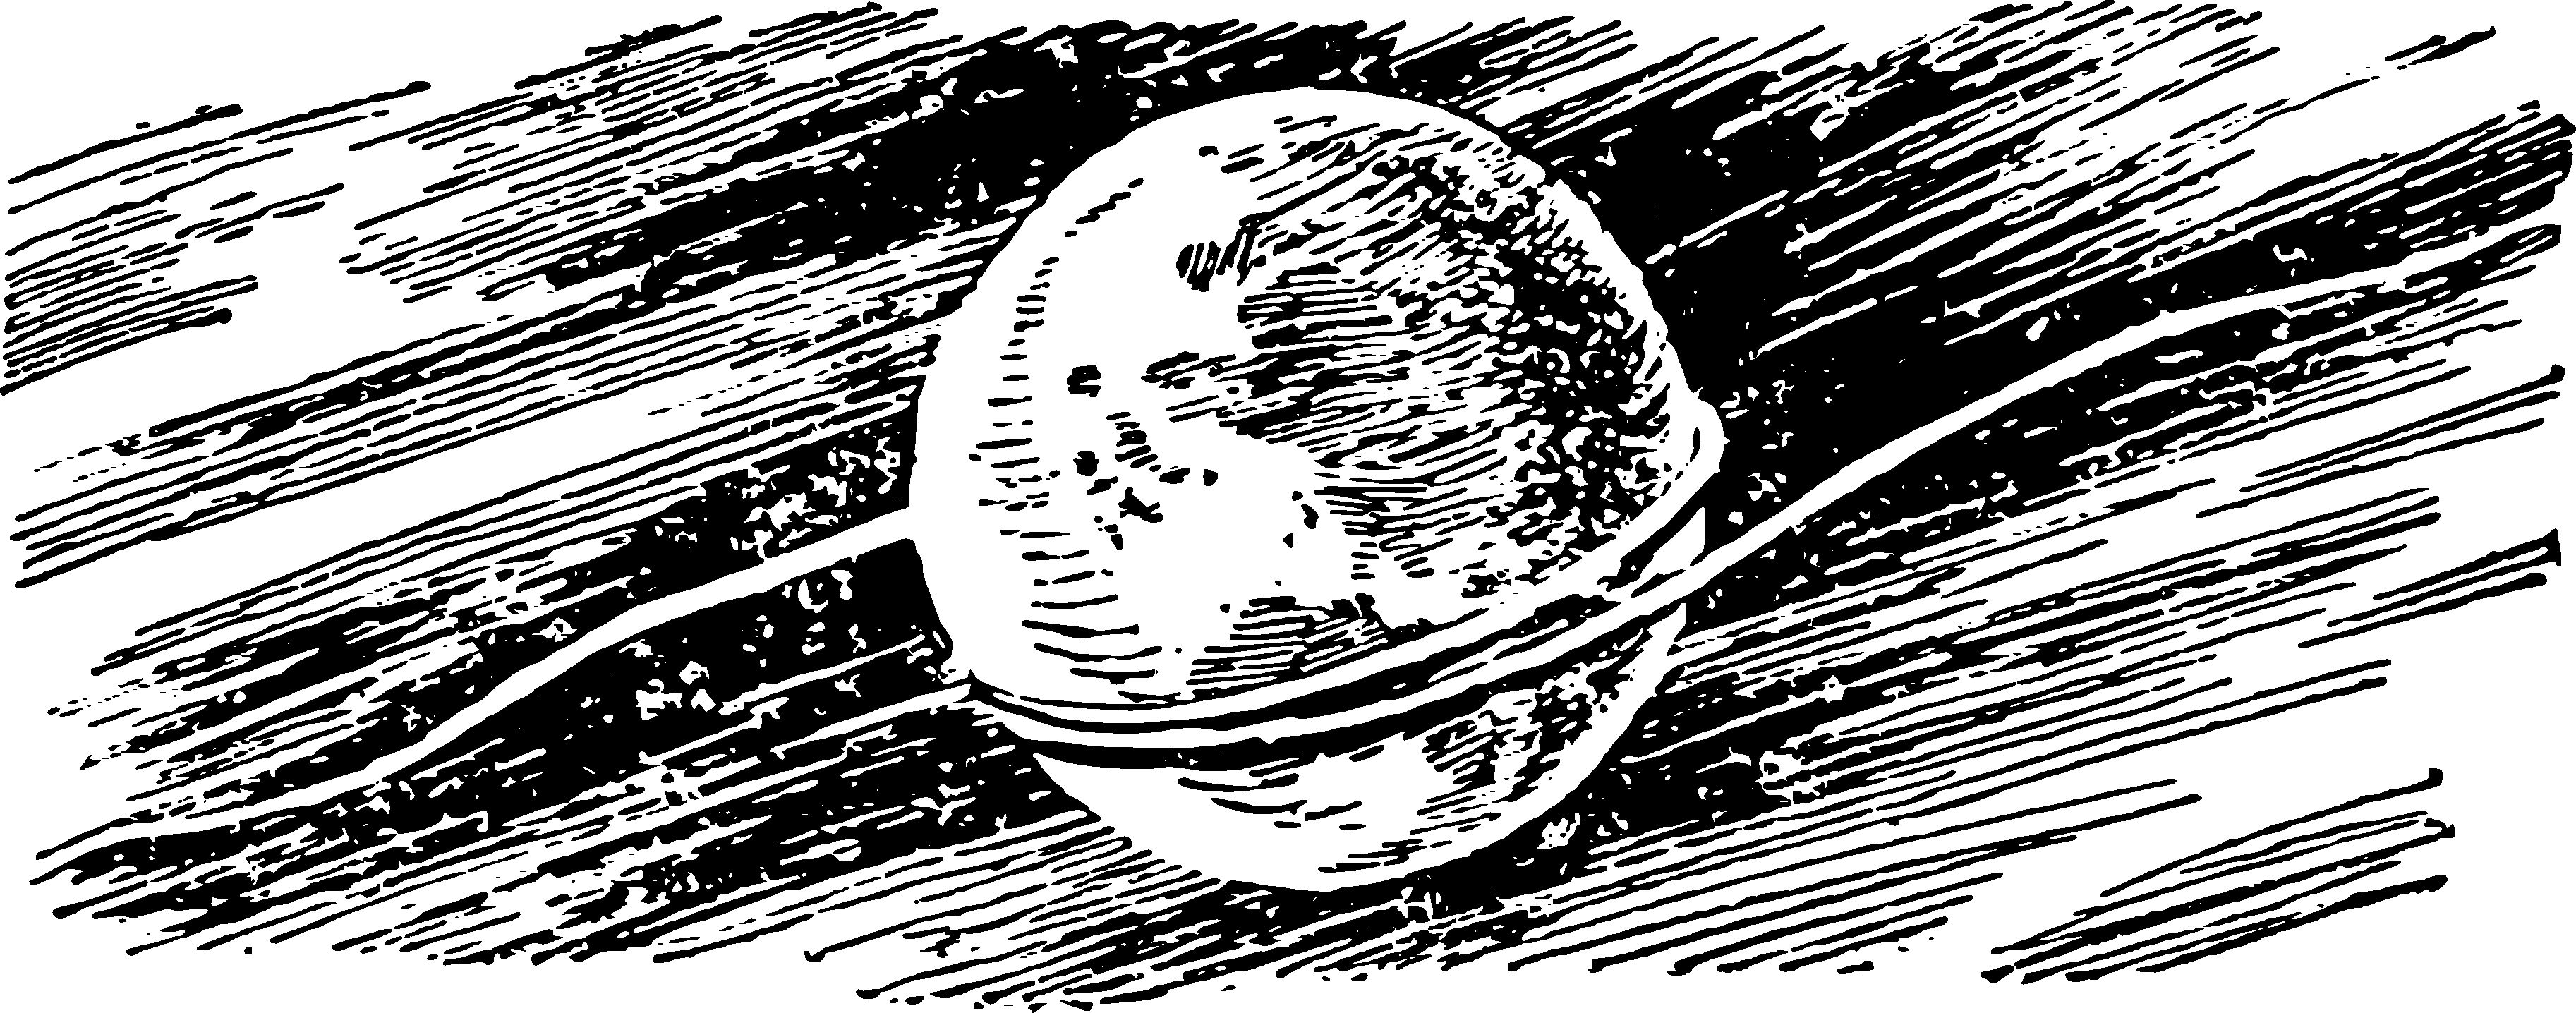
\includegraphics[width=1.2\textwidth]{figures/ch-09/fig-ch-09-head.pdf}\bigskip}

\chapter{Old And New About The Circle}
\label{ch-09}



\section{Practical geometry of the Egyptians and Romans}
\label{sec-9.1}

Any schoolchild can now calculate the circumference based on its diameter much more accurately than the wisest priest of the ancient land of pyramids or the most skilled architect of great Rome. The ancient Egyptians believed that the circumference was 3.16 times longer than the diameter, while the Romans believed it was 3.12 times longer. However, the correct ratio is 3.14159\dots{} Egyptian and Roman mathematicians established the ratio of the circumference to the diameter not through strict geometric calculation, as later mathematicians did, but simply through experience. But why did they make such errors? Couldn't they just stretch a piece of string around a circular object and then straighten the string to measure it?

Undoubtedly, they did just that, but it should not be assumed that such a method would necessarily yield good results. Imagine, for example, a vase with a round bottom with a diameter of \SI{100}{\milli\meter}. The circumference of the bottom should be \SI{314}{\milli\meter}. However, in practise, measuring with a string, you are unlikely to get this length: it is easy to make a mistake of one millimetre, and then $\pi$ will turn out to be equal to 3.13 or 3.15. And if you consider that the diameter of the vase cannot be measured perfectly accurately either, and that an error of \SI{1}{\milli\meter} is quite probable here too, then you will see that for $\pi$, quite wide limits are obtained between 
\begin{equation*}%
\frac{313}{101} \qand \frac{315}{99},
\end{equation*}
i.e., in decimal fractions, between 
\begin{equation*}%
3.09 \qand 3.18.
\end{equation*}
You see, by determining $\pi$ in this way, we can get a result that does not coincide with 3.14: once it's 3.1, another time 3.12, the third time 3.17, and so on. Among them, by chance, there may be 3.14, but in the eyes of the calculator, this number will not carry more weight than the others.

Such an empirical approach cannot provide a somewhat acceptable value for $\pi$. In this regard, it becomes more understandable why the ancient world did not know the correct ratio of the circumference to the diameter and why it took the genius of Archimedes to find the value of $3\,\frac{1}{7}$ for $\pi$ without measuring, relying solely on reasoning.



\section{``I know this and I remember it perfectly.''}

In the \emph{Algebra} of the ancient Arab mathematician Mohammed ibn-Musa, we read the following lines about calculating the circumference:
\begin{quote}
The best way is to multiply the diameter by $3\,\frac{1}{7}$. This is the fastest and easiest way. God knows the best. 
\end{quote}
Now we also know that Archimedes' number $3\,\frac{1}{7}$ does not perfectly express the ratio of the circumference to the diameter. It has been theoretically proven that this ratio cannot be expressed as any exact fraction. We can only write it with some approximation, which, however, far exceeds the accuracy required for the strictest demands of practical life. The mathematician Ludolph in the 16th century, in Leiden, had the patience to calculate $\pi$ with 35 decimal places and bequeathed to have this value for $\pi$ carved on his tombstone\sidenote{At that time, the notation $\pi$ was not yet in use: it was introduced only from the middle of the 18th century by the famous Russian academician and mathematician Leonard Pavlovich Euler.}! (see \figr{fig-123}).

Here it is: 
\begin{equation*}%
3.14159265358979323846264338327950288\dots{}
\end{equation*}
A certain Shanks in 1873 published a value of $\pi$ in which there were 707 decimal places after the comma! Such long numbers approximately expressing the value of $\pi$ have neither practical nor theoretical value. Only out of idleness and in pursuit of inflated ``records'' could there arise in our time a desire to "outdo" Shanks: in 1946-1947, Ferguson (Manchester City) and, independently of him, Weaver (from Washington) calculated 808 decimal places for the number $\pi$ and were pleased to find errors in Shanks's calculations starting from the 528th digit.

If, for example, we wished to calculate the length of the Earth's equator with an accuracy of \SI{1}{\centi\meter}, assuming that we know the length of its diameter precisely, it would be sufficient for us to take only 9 digits after the decimal point in the number $\pi$. And by taking twice as many digits (18), we could calculate the circumference with a precision of not more than \SI{0.0001}{\milli\meter} (100 times smaller than the thickness of a hair!) for a circle with a radius equal to the distance from the Earth to the Sun.

Our compatriot, the mathematician Grave, vividly demonstrated the absolute uselessness of even the first hundred decimal places of $\pi$. He calculated that if we imagine a sphere with a radius equal to the distance from the Earth to Sirius, i.e., a number of kilometres equal to 132 followed by ten zeros: \num{132d10}, and fill this sphere with microbes, placing one billion (\num{d10}) microbes in each cubic millimetre of the sphere, and then arrange all these microbes in a straight line so that the distance between each pair of adjacent microbes again equals the distance from Sirius to Earth, then, taking this fantastic segment as the diameter of a circle, it would be possible to calculate the length of the resulting gigantic circumference with microscopic precision — up to \SI{0.000001}{\milli\metre}, by using 100 digits after the decimal point in the number $\pi$. French astronomer Arago correctly observes in this regard that ``in terms of accuracy, we would gain nothing if there were a relationship between the circumference and the diameter expressed by a number with complete accuracy.''

For ordinary calculations involving $\pi$, it is sufficient to remember two digits after the decimal point (3.14), and for more precise calculations, four digits (3.1416: we take the last digit as 6 instead of 5 because the following digit is greater than 5).

Small poems or vivid phrases are better retained in memory than numbers, so special poems or individual phrases are invented to memorise some numerical value of $\pi$. In works of this kind of mathematical poetry, words are chosen so that the number of letters in each word sequentially coincides with the corresponding digit of the number $\pi$.

There is a famous poem in English -- in 13 words, hence providing 12 digits after the decimal point in the number $\pi$; in German -- in 24 words, and in French, in 30 words! (and there are even ones in 126 words).

They are curious but too large, cumbersome. Among the students, E. Y. Terskov, a mathematics teacher at one of the secondary schools in the Moscow region, enjoys popularity for inventing the following stanza:
\begin{quote}
«Это я знаю и помню прекрасно».\\
3     1 4   1  5    9 \dots{} \\
'I know this and remember it perfectly.' \\
\end{quote}


And one of his students, Elya Cherikover, with the resourcefulness typical of our schoolchildren, composed a witty, slightly ironic continuation:
\begin{quote}
«Пи многие знаки мне лишни, напрасны»,\\
2 6 5 3 5 9 26\\
'Pi, many digits are unnecessary for me, in vain,' \dots{}
\end{quote}
In total, a twelve-word couplet is obtained:

'I know this and remember it perfectly, Pi, many digits are unnecessary for me, in vain.'

The author of this book, not daring to invent a poem, in turn suggests a simple and also quite sufficient prose phrase:

«Что я знаю о круг» 'What do I know about circles?' — a question, secretly containing the answer; 3.1416.


%\vspace{2cm}

\begin{center}
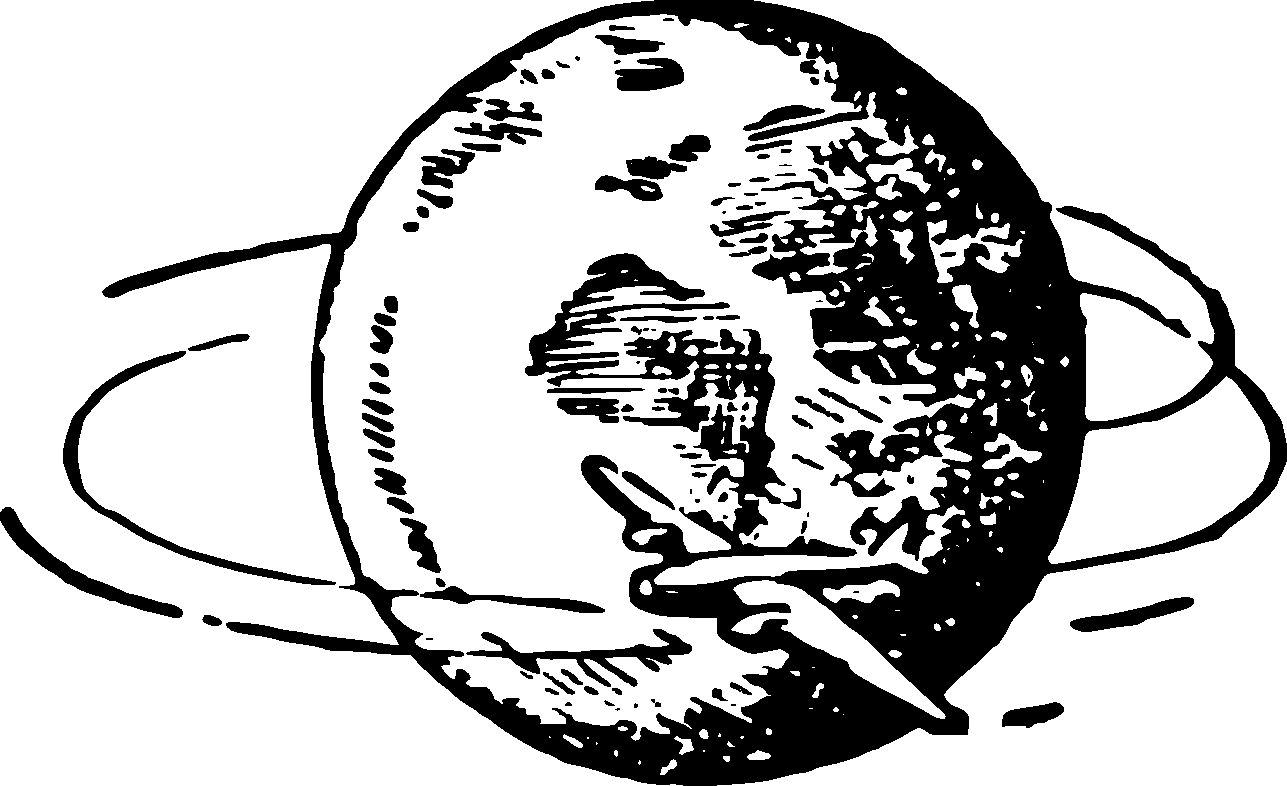
\includegraphics[width=0.3\textwidth]{figures/ch-09/fig-ch-09-tail.pdf}
\end{center}


















